\documentclass[crop, tikz]{standalone}

\usepackage[utf8]{inputenc}
% 'crop' is the default for v1.0, before it was 'preview'
%\usetikzlibrary{...}% tikz package already loaded by 'tikz' option

\usetikzlibrary{arrows}
\usetikzlibrary{decorations.markings}
\usetikzlibrary{patterns}
\usetikzlibrary{calc}

\begin{document}
	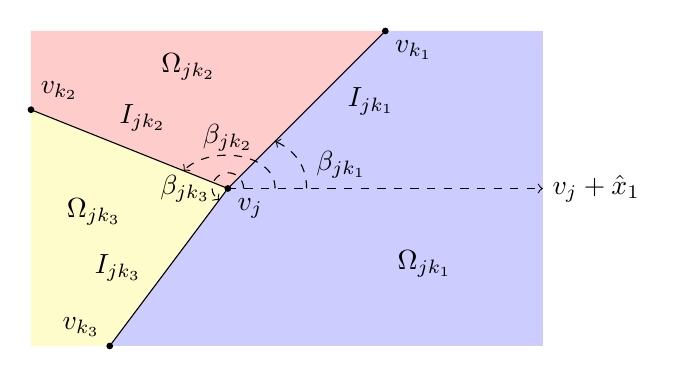
\begin{tikzpicture}[]
	
		%surrounding vertex coords
		\coordinate (vj) at (0,0);
		\coordinate (axis) at (4,0);
		\coordinate (v1) at (2,2);
		\coordinate (v2) at (-2.5,1);
		\coordinate (v3) at (-1.5,-2);
	
		%filldraw the bulk regions for ease?
		\filldraw[fill=blue!20!white, draw=none] (vj) -- (v3) -- (4,-2) -- (4,2) -- (v1) -- cycle;
		\filldraw[fill=red!20!white, draw=none] (vj) -- (v1) -- (-2.5,2) -- (v2) -- cycle;
		\filldraw[fill=yellow!20!white, draw=none] (vj) -- (v2) -- (-2.5,-2) -- (v3) --cycle;
		%bulk region labels
		\node[anchor=south] at (2.5,-1.25) {$\Omega_{jk_1}$};
		\node[anchor=south] at (-0.5,1.25) {$\Omega_{jk_2}$};
		\node[anchor=north] at (-1.70,0.0) {$\Omega_{jk_3}$};
	
		%draw vertices
		\filldraw[black] (vj) circle (1pt) node[anchor=north west] {$v_j$};
		\filldraw[black] (v1) circle (1pt) node[anchor=north west] {$v_{k_1}$};
		\filldraw[black] (v2) circle (1pt) node[anchor=south west] {$v_{k_2}$};
		\filldraw[black] (v3) circle (1pt) node[anchor=south east] {$v_{k_3}$};
	
		%reference axis
		\draw[dashed, ->] (vj) -- (axis) node[anchor=west] {$v_j + \hat{x}_1$};
	
		%connecting edges
		\draw (vj) -- (v1);
		\draw (vj) -- (v2);
		\draw (vj) -- (v3);
		%edge labels
		\node[anchor=north west] at ($(vj)!0.70!(v1)$) {$I_{jk_1}$};
		\node[anchor=south west] at ($(vj)!0.60!(v2)$) {$I_{jk_2}$};
		\node[anchor=south east] at ($(vj)!0.65!(v3)$) {$I_{jk_3}$};
	
		%angle examples
		\draw[dashed, ->] ($(vj)!0.25!(axis)$) to[out=90, in=-25] ($(vj)!0.3!(v1)$);
		\node[anchor=south west] at ($(vj)!0.25!(axis)$) {$\beta_{jk_1}$};
		\draw[dashed, ->] ($(vj)!0.15!(axis)$) to[out=90, in=45] ($(vj)!0.225!(v2)$);
		\node[anchor=south] at ($(vj)!0.35!(0,1)$) {$\beta_{jk_2}$};
		\draw[dashed] ($(vj)!0.05!(axis)$) to[out=90, in=0] ($(vj)!0.05!(0,4)$) to[out=180, in=90] ($(vj)!0.05!(-4,0)$);
		\draw[dashed, ->] ($(vj)!0.05!(-4,0)$) to[out=-90, in=135] ($(vj)!0.075!(v3)$);
		\node[anchor=east] at ($(vj)!0.025!(-4,0)$) {$\beta_{jk_3}$};
	
	\end{tikzpicture}
\end{document}